122. \begin{figure}[ht!]
\center{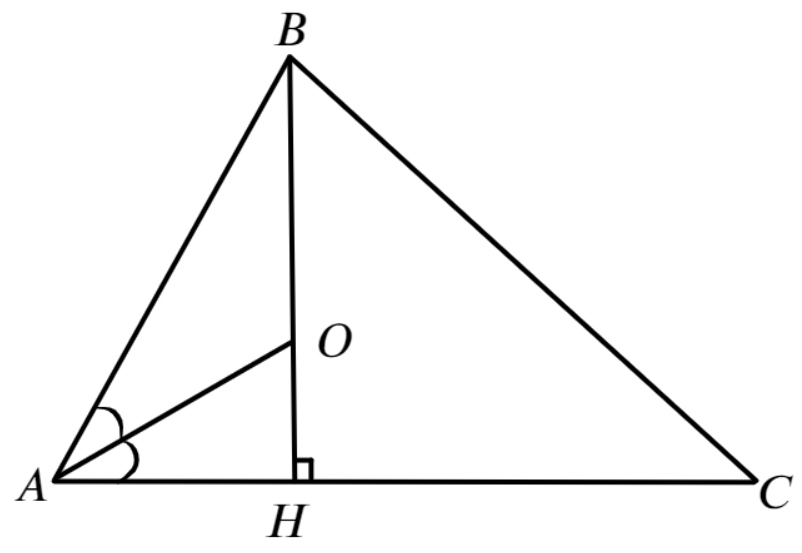
\includegraphics[scale=0.35]{g9-121.png}}
\end{figure}\\
По теореме синусов для треугольника $ABC$ получим $\cfrac{BC}{\sin(\angle A)}=2R,\ \cfrac{24}{\sin(\angle A)}=26,\ \sin(\angle A)=\cfrac{12}{13}.$
Тогда $\cos(\angle A)=\sqrt{1-\cfrac{144}{169}}=\cfrac{5}{13}=\cfrac{AH}{AB}$ (он положительный, так как в противном случае биссектриса угла $A$ не пересечёт высоту из точки $B$). По свойству основания биссектрисы имеем $\cfrac{AH}{AB}=\cfrac{OH}{OB}=\cfrac{5}{13},$ тогда $\cfrac{OB}{OH}=\cfrac{13}{5}.$\\
